\documentclass[a4paper,11pt]{article}
\usepackage{amsmath,amsthm,amsfonts,amssymb,bm} 
\usepackage{graphicx,psfrag} 
\usepackage{fancyhdr}
\usepackage{color} 
\usepackage{geometry}
\usepackage{multirow}
\usepackage{listings}
\usepackage{enumerate}
\usepackage{leftidx} 
\usepackage{mathrsfs} 

\usepackage{listings}
\usepackage{color}

\definecolor{mygreen}{rgb}{0,0.6,0}
\definecolor{mygray}{rgb}{0.5,0.5,0.5}
\definecolor{mymauve}{rgb}{0.58,0,0.82}

\lstset{ %
  backgroundcolor=\color{white},   % choose the background color; you must add \usepackage{color} or \usepackage{xcolor}
  basicstyle=\footnotesize,        % the size of the fonts that are used for the code
  breakatwhitespace=false,         % sets if automatic breaks should only happen at whitespace
  breaklines=true,                 % sets automatic line breaking
  captionpos=b,                    % sets the caption-position to bottom
  commentstyle=\color{mygreen},    % comment style
  deletekeywords={...},            % if you want to delete keywords from the given language
  escapeinside={\%*}{*)},          % if you want to add LaTeX within your code
  extendedchars=true,              % lets you use non-ASCII characters; for 8-bits encodings only, does not work with UTF-8
  keepspaces=true,                 % keeps spaces in text, useful for keeping indentation of code (possibly needs columns=flexible)
  keywordstyle=\color{blue},       % keyword style
  language=SQL,                 % the language of the code
  morekeywords={*,...},            % if you want to add more keywords to the set
  numbers=none,                    % where to put the line-numbers; possible values are (none, left, right)
  numbersep=5pt,                   % how far the line-numbers are from the code
  numberstyle=\tiny\color{mygray}, % the style that is used for the line-numbers
  rulecolor=\color{black},         % if not set, the frame-color may be changed on line-breaks within not-black text (e.g. comments (green here))
  showspaces=false,                % show spaces everywhere adding particular underscores; it overrides 'showstringspaces'
  showstringspaces=false,          % underline spaces within strings only
  showtabs=false,                  % show tabs within strings adding particular underscores
  stepnumber=2,                    % the step between two line-numbers. If it's 1, each line will be numbered
  stringstyle=\color{mymauve},     % string literal style
  tabsize=2,                       % sets default tabsize to 2 spaces
  title=\lstname                   % show the filename of files included with \lstinputlisting; also try caption instead of title
}

\geometry{left=3.17cm,right=3.17cm,top=2.54cm,bottom=2.54cm}

\begin{document}

\pagestyle{fancy}
\rfoot{\thepage}
\rhead{\bfseries Database System Concept}
\setlength{\parskip}{0.7ex plus0.2ex minus0.2ex}
\cfoot{\empty}
\lhead{\empty}


\title{Assignment 9}
\author{Qinglin Li, 5110309074}
\date{}
\maketitle

\headheight 3pt
\thispagestyle{fancy}
\section*{Problem 1}
\begin{enumerate}[a.]
\item 
\textbf{Hash-partitioning:}
Too many records with the same value for the hashing attribute, or a
poorly chosen hash function without the properties of randomness and
uniformity, can result in a skewed partition. To improve the situation, we
should experiment with better hashing functions for that relation.
\item
\textbf{Range-partitioning:}
Non-uniform distribution of values for the partitioning attribute (including
duplicate values for the partitioning attribute) which are not taken
into account by a bad partitioning vector is the main reason for skewed
partitions. Sorting the relation on the partitioning attribute and then dividing
it into n ranges with equal number of tuples per range will give a
good partitioning vector with very low skew.
\end{enumerate}

\section*{Problem 2}
The 5 partitions are
1-20, 21-30, 31-50, 51-75 and 76-100. \\
\textbf{Frequencies:}
\begin{enumerate}
\item 
1-20:$15+5=20$
\item 
21-30:$20$
\item
31-50:$10+10=20$
\item
51-75:$5+5+20/10*5=20$
\item
76-100:$20/10*5+5+5=20$
\end{enumerate}

\section*{Problem 3}
groupby rollup(a), rollup(b), rollup(c), rollup(d)

\section*{Problem 4}
\begin{lstlisting}
SELECT t, sum(c)
FROM (SELECT c, ntile(20) OVER (ORDER BY (a)) AS t FROM r) tt
GROUPBY t
\end{lstlisting}
\newpage
\section*{Problem 5}
\begin{lstlisting}
SELECT 1, COUNT(*)
FROM account
WHERE 3 * balance <= (SELECT MAX (balance) FROM account)
UNION
SELECT 2, COUNT (*)
FROM account
WHERE 3 * balance > (SELECT MAX(balance) FROM account)
	AND 1.5 * balance <= (SELECT MAX(balance) FROM account)
UNION
SELECT 3, COUNT (*)
FROM account
WHERE 1.5 * balance > (SELECT MAX(balance) FROM account)
\end{lstlisting}
\section*{Problem 6}
The information gain is the value in the node\\
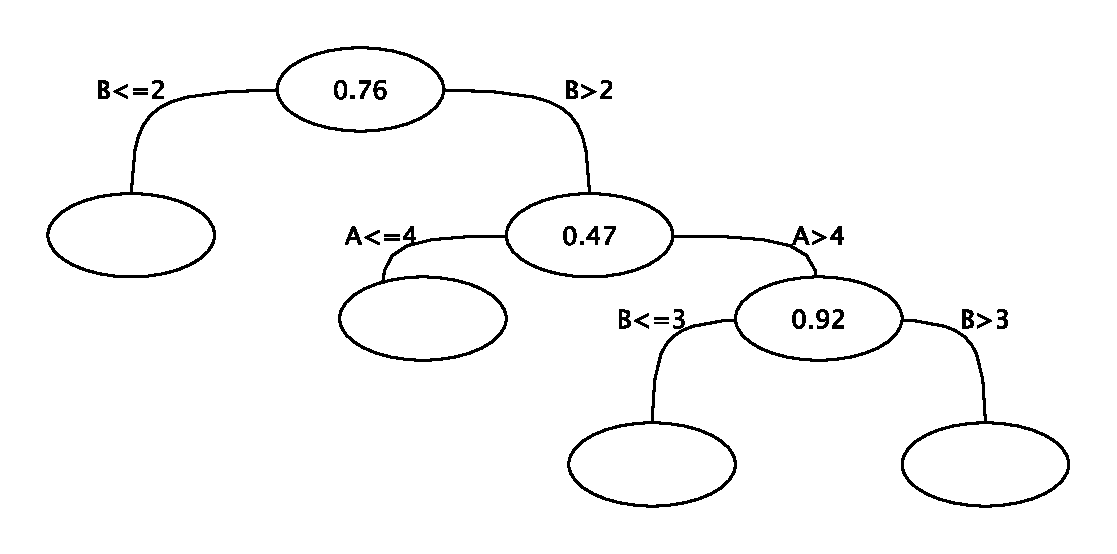
\includegraphics[scale=0.7]{fig.eps}
\end{document}

